

\chapter{Definiciones} % Main chapter title

\label{Definiciones} % Change X to a consecutive number; for referencing this chapter elsewhere, use \ref{ChapterX}

%----------------------------------------------------------------------------------------
%	SECTION 1
%----------------------------------------------------------------------------------------

\section{Aprendizaje automático}

Las técnicas de aprendizaje automático tienen como objetivo conseguir diferenciar automáticamente patrones usando algoritmos matemáticos. Se pueden distinguir dos tipos de técnicas: supervisadas y no supervisadas. En el aprendizaje supervisado se entrena al ordenador proporcionando ejemplos previamente etiquetados, de forma que el algoritmo usado debe encontrar las fronteras (o acercarse lo más posible) que separan los diferentes tipos de patrones. Las redes neuronales forman parte de este grupo. La figura~\ref{fig:frontera} simboliza la clasificación en un plano en dos dimensiones que se puede obtener con este tipo de algoritmo, donde dependiendo de los valores de entrada se determina a qué clase pertenece (X o +).

\begin{figure}[th]
\centering
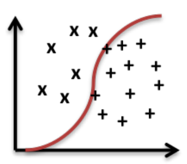
\includegraphics{Figures/figura_02.PNG}
\decoRule
\caption[Frontera de clasificación]{Frontera de clasificación de patrón \parencite{r63}.}
\label{fig:frontera}
\end{figure}


%-----------------------------------
%	SECTION 2
%-----------------------------------
\section{Redes neuronales}

En el campo del aprendizaje automático, las redes neuronales artificiales son una técnica computacional inspirada en la biología, en particular en el funcionamiento de las neuronas, sus conexiones y cómo éstas operan en red para su función. Cada neurona recibe un set de entradas las cuales a través de funciones de activación y parametrizaciones genera una salida, la cual podría convertirse en la entrada de otras neuronas en la red, las que en conjunto son capaces de generar un resultado. Los parámetros que poseen las neuronas se les llama pesos y sesgo (bias), los cuales se asocian a las conexiones de entrada. Estos parámetros son utilizados por su función de activación para generar la salida a partir de los datos de entrada. La figura~\ref{fig:neurona} representa el funcionamiento de una neurona artificial.

\begin{figure}[th]
\centering
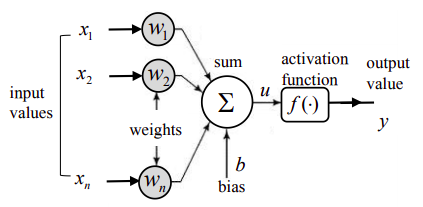
\includegraphics[scale = 1.1]{Figures/figura_03.PNG}
\decoRule
\caption[Neurona]{Neurona artificial \parencite{r64}.}
\label{fig:neurona}
\end{figure}

La salida de la red de neuronas representa posibles resultados de clasificación asociados a un problema. Una red neuronal artificial se compone de capas de neuronas las cuales se conectan entre sí como lo indica la figura~\ref{fig:red}. En la figura las neuronas agrupadas verticalmente representan una capa, cada neurona se conecta con todas las neuronas de la capa anterior y las de la capa siguiente. Cuando se posee al menos una capa oculta, el algoritmo usa arquitecturas computacionales que admiten transformaciones no lineales múltiples e iterativas de datos expresados en forma matricial o tensorial \parencite{r1}

\begin{figure}[th]
\centering
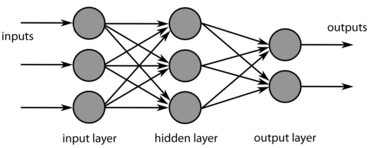
\includegraphics[scale = 1.1]{Figures/figura_04.PNG}
\decoRule
\caption[Neurona]{Red neuronal artificial. Arquitectura simplificada de Perceptrón multicapa \parencite{r13}.}
\label{fig:red}
\end{figure}

Estas redes antes de ser puestas en operación se prepara de la siguiente manera:

\begin{enumerate}
\item Topología de la red: Se busca identificar e implementar topologías óptimas en cuanto a cantidad de capas y neuronas por capas.
\item Parametrización de neuronas: Las redes son entrenadas de manera de conseguir acercarse a la mejor parametrización de pesos por conexión entre neuronas. Para esto se debe contar con una gran cantidad de datos que estén previamente etiquetados, de esta manera se entrena la red ajustando los pesos de cada conexión haciendo tender la red a clasificar correctamente los datos de entrenamiento. A esta técnica en el aprendizaje automático se le llama aprendizaje supervisado, ya que se cuenta con datos de entrada y sus respectivas etiquetas (correcta clasificación) que permite entrenar y validar la eficacia de la red (en cuanto a aciertos).
\item Generalización: Se debe tener precaución respecto a que la red no sobre aprenda. Esto quiere decir que clasifique con un grado alto de exactitud los datos de entrenamiento, pero no así con datos de entrada no pertenecientes a los usados en el entrenamiento.
\end{enumerate}


\section{Redes de aprendizaje profundo}

El aprendizaje profundo es una rama del aprendizaje automático que permite que los modelos computacionales compuestos por múltiples capas de procesamiento con alto nivel de abstracción aprendan de la experiencia y perciban el mundo en términos de jerarquía de conceptos. Utiliza un algoritmo de backpropagation para descubrir detalles intrincados en grandes conjuntos de datos con el fin de calcular la representación de datos en cada capa a partir de la representación en la capa anterior \parencite{r36}. 
Los algoritmos de aprendizaje profundo contrastan con los algoritmos de aprendizaje poco profundo por el número de capas aplicadas a la señal mientras se propaga desde la capa de entrada a la capa de salida. No existe un estándar de facto para el número de capas que convierte a un algoritmo en profundo, pero la mayoría de investigadores en el campo considera que el aprendizaje profundo implica al menos dos capas ocultas \parencite{r2}. Este tipo de algoritmo permite obtener una gran efectividad en la clasificación y ha sido ampliamente utilizad en los últimos años. La figura~\ref{fig:deep} muestra la arquitectura de una red neuronal profunda.

\begin{figure}[th]
\centering
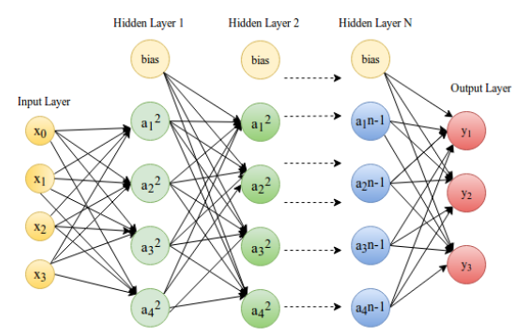
\includegraphics[scale = 1.1]{Figures/figura_05.PNG}
\decoRule
\caption[Neurona]{Red neuronal profunda \parencite{r7}.}
\label{fig:deep}
\end{figure}

Las redes neuronales artificiales no son totalmente confiables, sus salidas no corresponden a algoritmos matemáticos exactos y algunas de sus salidas son erróneas. Estas son entrenadas con grandes volúmenes de datos, de los cuales adquiere conocimiento que utiliza para generalizar sobre nuevas muestras desconocidas para el clasificador. La generalización no resulta eficaz en el total de los casos, pero se considera buena mientras más se acerque al 100\%. En este caso, los fallos se presentan principalmente cuando su entrada es muy distinta a los datos con la que la red fue entrenada.


\section{Visión artificial}

La visión artificial o visión por ordenador es una disciplina científica que incluye métodos para adquirir, procesar, analizar y comprender las imágenes del mundo real con el fin de producir información numérica o simbólica para que puedan ser tratados por un ordenador. Tal y como los humanos usamos nuestros ojos y cerebros para comprender el mundo que nos rodea, la visión artificial trata de producir el mismo efecto para que los ordenadores puedan percibir y comprender una imagen o secuencia de imágenes y actuar según convenga en una determinada situación.
A la hora de aplicar los conceptos teóricos de la visión por ordenador encontraremos siempre interferencias y problemas relacionados con el mundo que nos rodea. Esto es por el mero hecho de que nuestro mundo no es perfecto y los aparatos de medición y captura tampoco lo son. Estos introducen siempre (a mayor o menor cantidad) una distorsión o ruido que contamina la muestra o imagen con la que deseamos trabajar.

\subsection{Redes convolutivas}

Una de las aplicaciones más extendidas de las redes neuronales es la clasificación de imágenes, ya que en la última década ha generado excelentes resultados, llegando a ser muy similar a la clasificación de la vista humana en ciertos contextos. 
Las redes convolutivas son una técnica de las redes neuronales que contiene varias capas ocultas especializadas y con una jerarquía. Las primeras capas pueden detectar líneas curvas y se van especializando hasta llegar a capas más profundas que reconocen formas complejas como un rostro o la silueta de un animal. Este tipo de red neuronal artificial se inspira en el funcionamiento de los campos receptivos de las neuronas en la corteza visual primaria de un cerebro biológico. 

\subsubsection{Entrada de datos}

Las imágenes se transforman en matrices de datos, en donde cada pixel en la foto podría tener 3 dimensiones, según la nomenclatura RGB (Composición del color en términos de la intensidad de los colores) con valores entre 0 y 255. Estos valores a menudo se normalizan para obtener datos entre 0 y 1.  
Por otro lado es recomendable realizar ciertas modificaciones a la imagen de entrada de modo de mejorar la asertividad de la clasificación, generando desde las imágenes de entrada nuevas imágenes producto de rotaciones, acercamientos, traslaciones o de invertir la imagen en algún eje. Esto ayuda a que la red generalice de mejor forma, es decir que pueda clasificar imágenes nuevas distintas a las utilizadas en el entrenamiento.

\subsubsection{Procesamiento}

La figura~\ref{fig:convolutiva} muestra un ejemplo del preprocesamiento de redes convolutivas en donde se extraen las características principales de la imagen para luego ser procesada por una red neuronal como las presentadas previamente (clasificación).

\begin{figure}[th]
\centering
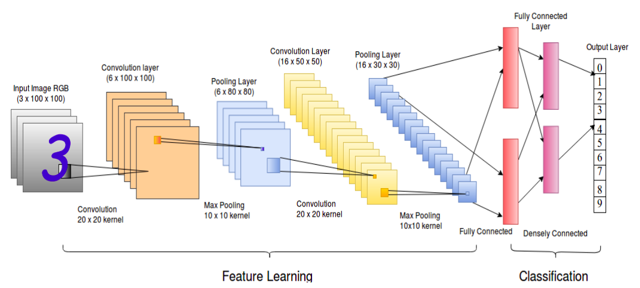
\includegraphics[scale = 0.9]{Figures/figura_06.PNG}
\decoRule
\caption[convolutiva]{Red neuronal convolutiva (CNN) \parencite{r7}.}
\label{fig:convolutiva}
\end{figure}

\subsubsection{Convolución}

Sobre la imagen de entrada se aplican distintos tipos de filtros llamados kernels. La figura~\ref{fig:kernel} muestra una convolución en donde cada píxel de salida es una combinación lineal de los pixeles de entrada. En la convolución se realizan operaciones de productos y sumas entre la capa de partida y los n filtros (o kernel) que genera un mapa de características. Las características extraídas corresponden a cada posible ubicación del filtro en la imagen original. La ventaja es que el mismo filtro sirve para extraer la misma característica en cualquier parte de la entrada, con esto se consigue reducir el número de conexiones y el número de parámetros a entrenar en comparación con una red multicapa de conexión total.

\begin{figure}[th]
\centering
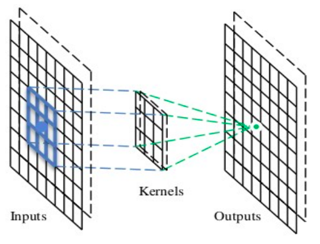
\includegraphics{Figures/figura_07.PNG}
\decoRule
\caption[convolutiva]{Convolución \parencite{r7}.}
\label{fig:kernel}
\end{figure}

\section{Flujo de procesamiento en aprendizaje automático}

Los sistemas de aprendizaje automático poseen un flujo de operación generalizado \parencite{r40} en el cual se puede representar la mayoría de los sistemas en los que se implementa. Este flujo se muestra en la figura~\ref{fig:flujo} en donde un objeto del dominio físico es representado digitalmente a través de cámaras, sensores, eventos de red u otro hardware. Luego la información es procesada en el modelo de aprendizaje automático, el cual entrega una salida, una probabilidad de clasificación u otro tipo de respuesta. El dominio físico recibe esta respuesta y la utiliza para ejecutar alguna acción, como sería el frenar en el caso de un coche de conducción automática frente a una señalética de tránsito. 

\begin{figure}[th]
\centering
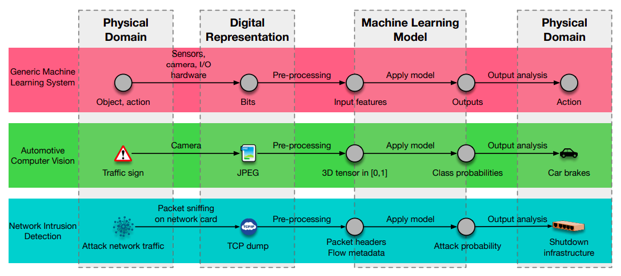
\includegraphics [scale = 0.85]{Figures/figura_08.PNG}
\decoRule
\caption[Flujo genérico] {Flujo genérico de Procesamiento de datos Aprendizaje automático \parencite{r40}.}
\label{fig:flujo}
\end{figure}

\section{Redes generativas con adversario (GAN)}
Las redes generativas con adversario o GAN son redes profundas que compiten en un juego de optimización, en donde existen dos jugadores como se muestran en la figura~\ref{fig:gan2}. Un jugador corresponde a una red neuronal con el rol de “generador”, cuyo objetivo es generar datos sintéticos a partir de una entrada aleatoria, que serán consumidos por el segundo jugador que corresponde a una red neuronal con el rol de discriminador. El discriminador recibe entradas reales (de algún conjunto de datos existente) y sintéticas (generadas por el generador), el discriminador será entrenado en clasificar correctamente las entradas reales y las falsas (sintéticas), mientras el generador será optimizado para crear datos más parecidos a los reales para hacer fallar al discriminador. El procedimiento finaliza cuando el discriminador no logra identificar las entradas sintéticas \parencite{r42}. La figura~\ref{fig:gan1} muestra imágenes creadas por el generador, con excepción de la columna enmarcada en amarillo que corresponde a imágenes reales del conjunto de datos, más similar a las sintéticas, presentada para demostrar que el modelo no memorizó las imágenes, sino que creó nuevas. Una de las aplicaciones de este modelo es la creación de imágenes para aumentar los datos de los entrenamientos y así mejorar la exactitud de algún modelo clasificador.

\begin{figure}[th]
\centering
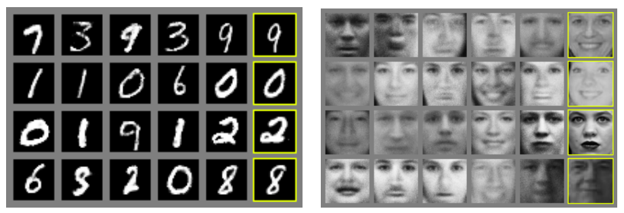
\includegraphics [scale = 0.85]{Figures/figura_09.PNG}
\decoRule
\caption[GAN] {Imágenes creadas por un modelo generador GAN (sintéticas). En amarillo imágenes reales del conjunto de datos \parencite{r42}.}
\label{fig:gan1}
\end{figure}

\begin{figure}[th]
\centering
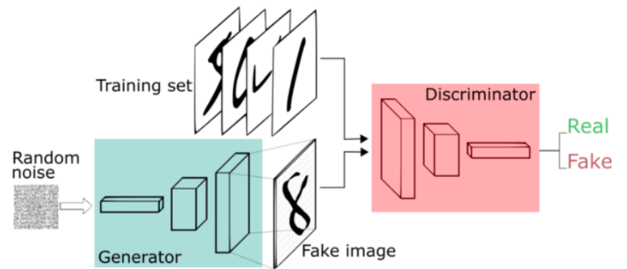
\includegraphics [scale = 0.85]{Figures/figura_10.PNG}
\decoRule
\caption[GAN] {Operación redes generativas con adversario \parencite{r41}.}
\label{fig:gan2}
\end{figure}

Existen variaciones al modelo GAN, como CycleGAN \parencite{r48} con la cual es posible realizar una traducción de imagen a imagen, mapeando en una imagen las características de otra. La figura~\ref{fig:gan3} muestra los resultados obtenidos en un estudio \parencite{r48} en donde una red generadora crea una imagen sintética de estilo fotográfico a partir de una pintura de óleo de Monet (parte superior izquierda), como también transformar imágenes de caballos en cebras o paisajes invernales a veraniegas. 


\begin{figure}[th]
\centering
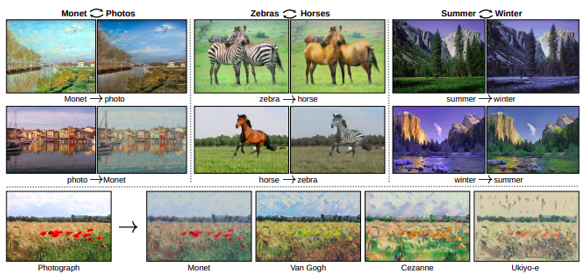
\includegraphics [scale = 0.85]{Figures/figura_11.PNG}
\decoRule
\caption[CycleGAN] {CycleGAN para la traducción de una imagen a otra \parencite{r48}.}
\label{fig:gan3}
\end{figure}

El modelo posee dos funciones de mapeo (una para cada clase de imágenes, ejemplo: caballos y cebras) y también sus respectivos discriminadores Dy y Dx. Dy evalúa si las traducciones de G(X) son indistinguibles a las imágenes del dominio Y, y viceversa Dx con F(Y). Esto en un ciclo el cual comienza con G(X) luego la imagen traducida es vuelta a su estilo original con F(Y) y se ajustan las redes de acuerdo a la pérdida entre la imagen original y la revertida como se indica en la figura~\ref{fig:gan4}.

\begin{figure}[th]
\centering
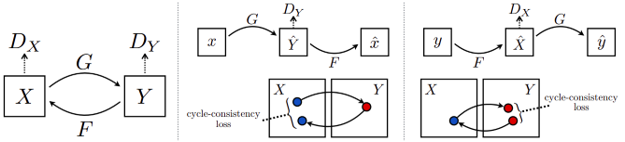
\includegraphics [scale = 0.85]{Figures/figura_12.PNG}
\decoRule
\caption[CycleGAN] {Procedimientos del método CycleGAN \parencite{r48}.}
\label{fig:gan4}
\end{figure}

La figura~\ref{fig:gan5} muestra el ciclo de traducción de imágenes, la primera columna son las imágenes originales, la segunda es la traducida y la tercera es la reconstituida a partir de la traducida. Una de las aplicaciones de este modelo es en el campo de los GIS (sistemas de información geográfica) en el cual como se observa en la última fila de la figura~\ref{fig:gan5}, es posible crear imágenes del estilo de la aplicación de google maps desde fotografías satelitales.

\begin{figure}[th]
\centering
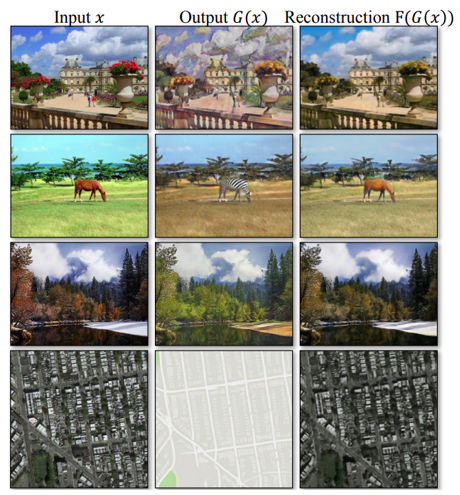
\includegraphics [scale = 0.85]{Figures/figura_13.PNG}
\decoRule
\caption[CycleGAN] {CycleGAN. Traducción de imágenes y reconstrucción de originales \parencite{r48}.}
\label{fig:gan5}
\end{figure}